%!TEX spellcheck = en_US

%% bare_jrnl.tex
%% V1.4b
%% 2015/08/26
%% by Michael Shell
%% see http://www.michaelshell.org/
%% for current contact information.
%%
%% This is a skeleton file demonstrating the use of IEEEtran.cls
%% (requires IEEEtran.cls version 1.8b or later) with an IEEE
%% journal paper.
%%
%% Support sites:
%% http://www.michaelshell.org/tex/ieeetran/
%% http://www.ctan.org/pkg/ieeetran
%% and
%% http://www.ieee.org/


%%*************************************************************************
%% Legal Notice:
%% This code is offered as-is without any warranty either expressed or
%% implied; without even the implied warranty of MERCHANTABILITY or
%% FITNESS FOR A PARTICULAR PURPOSE! 
%% User assumes all risk.
%% In no event shall the IEEE or any contributor to this code be liable for
%% any damages or losses, including, but not limited to, incidental,
%% consequential, or any other damages, resulting from the use or misuse
%% of any information contained here.
%%
%% All comments are the opinions of their respective authors and are not
%% necessarily endorsed by the IEEE.
%%
%% This work is distributed under the LaTeX Project Public License (LPPL)
%% ( http://www.latex-project.org/ ) version 1.3, and may be freely used,
%% distributed and modified. A copy of the LPPL, version 1.3, is included
%% in the base LaTeX documentation of all distributions of LaTeX released
%% 2003/12/01 or later.
%% Retain all contribution notices and credits.
%% ** Modified files should be clearly indicated as such, including  **
%% ** renaming them and changing author support contact information. **
%%*************************************************************************


% *** Authors should verify (and, if needed, correct) their LaTeX system  ***
% *** with the testflow diagnostic prior to trusting their LaTeX platform ***
% *** with production work. The IEEE's font choices and paper sizes can   ***
% *** trigger bugs that do not appear when using other class files.       ***                          ***
% The testflow support page is at:
% http://www.michaelshell.org/tex/testflow/

%
\documentclass[conference]{IEEEtran}
%
% If IEEEtran.cls has not been installed into the LaTeX system files,
% manually specify the path to it like:
% \documentclass[journal]{../sty/IEEEtran}

%\input epsf
\usepackage{graphicx}
\usepackage{hyperref}
\usepackage{graphicx}
\usepackage{amssymb}
\usepackage{amsmath}
\usepackage[super]{nth}
\usepackage{multicol}
\usepackage[T1]{fontenc}
\usepackage{textcomp}
\usepackage{gensymb}


% Some very useful LaTeX packages include:
% (uncomment the ones you want to load)


% *** MISC UTILITY PACKAGES ***
%
%\usepackage{ifpdf}
% Heiko Oberdiek's ifpdf.sty is very useful if you need conditional
% compilation based on whether the output is pdf or dvi.
% usage:
% \ifpdf
%   % pdf code
% \else
%   % dvi code
% \fi
% The latest version of ifpdf.sty can be obtained from:
% http://www.ctan.org/pkg/ifpdf
% Also, note that IEEEtran.cls V1.7 and later provides a builtin
% \ifCLASSINFOpdf conditional that works the same way.
% When switching from latex to pdflatex and vice-versa, the compiler may
% have to be run twice to clear warning/error messages.






% *** CITATION PACKAGES ***
%
%\usepackage{cite}
% cite.sty was written by Donald Arseneau
% V1.6 and later of IEEEtran pre-defines the format of the cite.sty package
% \cite{} output to follow that of the IEEE. Loading the cite package will
% result in citation numbers being automatically sorted and properly
% "compressed/ranged". e.g., [1], [9], [2], [7], [5], [6] without using
% cite.sty will become [1], [2], [5]--[7], [9] using cite.sty. cite.sty's
% \cite will automatically add leading space, if needed. Use cite.sty's
% noadjust option (cite.sty V3.8 and later) if you want to turn this off
% such as if a citation ever needs to be enclosed in parenthesis.
% cite.sty is already installed on most LaTeX systems. Be sure and use
% version 5.0 (2009-03-20) and later if using hyperref.sty.
% The latest version can be obtained at:
% http://www.ctan.org/pkg/cite
% The documentation is contained in the cite.sty file itself.






% *** GRAPHICS RELATED PACKAGES ***
%
\ifCLASSINFOpdf
  % \usepackage[pdftex]{graphicx}
  % declare the path(s) where your graphic files are
  % \graphicspath{{../pdf/}{../jpeg/}}
  % and their extensions so you won't have to specify these with
  % every instance of \includegraphics
  % \DeclareGraphicsExtensions{.pdf,.jpeg,.png}
\else
  % or other class option (dvipsone, dvipdf, if not using dvips). graphicx
  % will default to the driver specified in the system graphics.cfg if no
  % driver is specified.
  % \usepackage[dvips]{graphicx}
  % declare the path(s) where your graphic files are
  % \graphicspath{{../eps/}}
  % and their extensions so you won't have to specify these with
  % every instance of \includegraphics
  % \DeclareGraphicsExtensions{.eps}
\fi
% graphicx was written by David Carlisle and Sebastian Rahtz. It is
% required if you want graphics, photos, etc. graphicx.sty is already
% installed on most LaTeX systems. The latest version and documentation
% can be obtained at: 
% http://www.ctan.org/pkg/graphicx
% Another good source of documentation is "Using Imported Graphics in
% LaTeX2e" by Keith Reckdahl which can be found at:
% http://www.ctan.org/pkg/epslatex
%
% latex, and pdflatex in dvi mode, support graphics in encapsulated
% postscript (.eps) format. pdflatex in pdf mode supports graphics
% in .pdf, .jpeg, .png and .mps (metapost) formats. Users should ensure
% that all non-photo figures use a vector format (.eps, .pdf, .mps) and
% not a bitmapped formats (.jpeg, .png). The IEEE frowns on bitmapped formats
% which can result in "jaggedy"/blurry rendering of lines and letters as
% well as large increases in file sizes.
%
% You can find documentation about the pdfTeX application at:
% http://www.tug.org/applications/pdftex





% *** MATH PACKAGES ***
%
%\usepackage{amsmath}
% A popular package from the American Mathematical Society that provides
% many useful and powerful commands for dealing with mathematics.
%
% Note that the amsmath package sets \interdisplaylinepenalty to 10000
% thus preventing page breaks from occurring within multiline equations. Use:
%\interdisplaylinepenalty=2500
% after loading amsmath to restore such page breaks as IEEEtran.cls normally
% does. amsmath.sty is already installed on most LaTeX systems. The latest
% version and documentation can be obtained at:
% http://www.ctan.org/pkg/amsmath





% *** SPECIALIZED LIST PACKAGES ***
%
%\usepackage{algorithmic}
% algorithmic.sty was written by Peter Williams and Rogerio Brito.
% This package provides an algorithmic environment fo describing algorithms.
% You can use the algorithmic environment in-text or within a figure
% environment to provide for a floating algorithm. Do NOT use the algorithm
% floating environment provided by algorithm.sty (by the same authors) or
% algorithm2e.sty (by Christophe Fiorio) as the IEEE does not use dedicated
% algorithm float types and packages that provide these will not provide
% correct IEEE style captions. The latest version and documentation of
% algorithmic.sty can be obtained at:
% http://www.ctan.org/pkg/algorithms
% Also of interest may be the (relatively newer and more customizable)
% algorithmicx.sty package by Szasz Janos:
% http://www.ctan.org/pkg/algorithmicx




% *** ALIGNMENT PACKAGES ***
%
%\usepackage{array}
% Frank Mittelbach's and David Carlisle's array.sty patches and improves
% the standard LaTeX2e array and tabular environments to provide better
% appearance and additional user controls. As the default LaTeX2e table
% generation code is lacking to the point of almost being broken with
% respect to the quality of the end results, all users are strongly
% advised to use an enhanced (at the very least that provided by array.sty)
% set of table tools. array.sty is already installed on most systems. The
% latest version and documentation can be obtained at:
% http://www.ctan.org/pkg/array


% IEEEtran contains the IEEEeqnarray family of commands that can be used to
% generate multiline equations as well as matrices, tables, etc., of high
% quality.




% *** SUBFIGURE PACKAGES ***
%\ifCLASSOPTIONcompsoc
%  \usepackage[caption=false,font=normalsize,labelfont=sf,textfont=sf]{subfig}
%\else
%  \usepackage[caption=false,font=footnotesize]{subfig}
%\fi
% subfig.sty, written by Steven Douglas Cochran, is the modern replacement
% for subfigure.sty, the latter of which is no longer maintained and is
% incompatible with some LaTeX packages including fixltx2e. However,
% subfig.sty requires and automatically loads Axel Sommerfeldt's caption.sty
% which will override IEEEtran.cls' handling of captions and this will result
% in non-IEEE style figure/table captions. To prevent this problem, be sure
% and invoke subfig.sty's "caption=false" package option (available since
% subfig.sty version 1.3, 2005/06/28) as this is will preserve IEEEtran.cls
% handling of captions.
% Note that the Computer Society format requires a larger sans serif font
% than the serif footnote size font used in traditional IEEE formatting
% and thus the need to invoke different subfig.sty package options depending
% on whether compsoc mode has been enabled.
%
% The latest version and documentation of subfig.sty can be obtained at:
% http://www.ctan.org/pkg/subfig




% *** FLOAT PACKAGES ***
%
%\usepackage{fixltx2e}
% fixltx2e, the successor to the earlier fix2col.sty, was written by
% Frank Mittelbach and David Carlisle. This package corrects a few problems
% in the LaTeX2e kernel, the most notable of which is that in current
% LaTeX2e releases, the ordering of single and double column floats is not
% guaranteed to be preserved. Thus, an unpatched LaTeX2e can allow a
% single column figure to be placed prior to an earlier double column
% figure.
% Be aware that LaTeX2e kernels dated 2015 and later have fixltx2e.sty's
% corrections already built into the system in which case a warning will
% be issued if an attempt is made to load fixltx2e.sty as it is no longer
% needed.
% The latest version and documentation can be found at:
% http://www.ctan.org/pkg/fixltx2e


%\usepackage{stfloats}
% stfloats.sty was written by Sigitas Tolusis. This package gives LaTeX2e
% the ability to do double column floats at the bottom of the page as well
% as the top. (e.g., "\begin{figure*}[!b]" is not normally possible in
% LaTeX2e). It also provides a command:
%\fnbelowfloat
% to enable the placement of footnotes below bottom floats (the standard
% LaTeX2e kernel puts them above bottom floats). This is an invasive package
% which rewrites many portions of the LaTeX2e float routines. It may not work
% with other packages that modify the LaTeX2e float routines. The latest
% version and documentation can be obtained at:
% http://www.ctan.org/pkg/stfloats
% Do not use the stfloats baselinefloat ability as the IEEE does not allow
% \baselineskip to stretch. Authors submitting work to the IEEE should note
% that the IEEE rarely uses double column equations and that authors should try
% to avoid such use. Do not be tempted to use the cuted.sty or midfloat.sty
% packages (also by Sigitas Tolusis) as the IEEE does not format its papers in
% such ways.
% Do not attempt to use stfloats with fixltx2e as they are incompatible.
% Instead, use Morten Hogholm'a dblfloatfix which combines the features
% of both fixltx2e and stfloats:
%
% \usepackage{dblfloatfix}
% The latest version can be found at:
% http://www.ctan.org/pkg/dblfloatfix




%\ifCLASSOPTIONcaptionsoff
%  \usepackage[nomarkers]{endfloat}
% \let\MYoriglatexcaption\caption
% \renewcommand{\caption}[2][\relax]{\MYoriglatexcaption[#2]{#2}}
%\fi
% endfloat.sty was written by James Darrell McCauley, Jeff Goldberg and 
% Axel Sommerfeldt. This package may be useful when used in conjunction with 
% IEEEtran.cls'  captionsoff option. Some IEEE journals/societies require that
% submissions have lists of figures/tables at the end of the paper and that
% figures/tables without any captions are placed on a page by themselves at
% the end of the document. If needed, the draftcls IEEEtran class option or
% \CLASSINPUTbaselinestretch interface can be used to increase the line
% spacing as well. Be sure and use the nomarkers option of endfloat to
% prevent endfloat from "marking" where the figures would have been placed
% in the text. The two hack lines of code above are a slight modification of
% that suggested by in the endfloat docs (section 8.4.1) to ensure that
% the full captions always appear in the list of figures/tables - even if
% the user used the short optional argument of \caption[]{}.
% IEEE papers do not typically make use of \caption[]'s optional argument,
% so this should not be an issue. A similar trick can be used to disable
% captions of packages such as subfig.sty that lack options to turn off
% the subcaptions:
% For subfig.sty:
% \let\MYorigsubfloat\subfloat
% \renewcommand{\subfloat}[2][\relax]{\MYorigsubfloat[]{#2}}
% However, the above trick will not work if both optional arguments of
% the \subfloat command are used. Furthermore, there needs to be a
% description of each subfigure *somewhere* and endfloat does not add
% subfigure captions to its list of figures. Thus, the best approach is to
% avoid the use of subfigure captions (many IEEE journals avoid them anyway)
% and instead reference/explain all the subfigures within the main caption.
% The latest version of endfloat.sty and its documentation can obtained at:
% http://www.ctan.org/pkg/endfloat
%
% The IEEEtran \ifCLASSOPTIONcaptionsoff conditional can also be used
% later in the document, say, to conditionally put the References on a 
% page by themselves.




% *** PDF, URL AND HYPERLINK PACKAGES ***
%
%\usepackage{url}
% url.sty was written by Donald Arseneau. It provides better support for
% handling and breaking URLs. url.sty is already installed on most LaTeX
% systems. The latest version and documentation can be obtained at:
% http://www.ctan.org/pkg/url
% Basically, \url{my_url_here}.




% *** Do not adjust lengths that control margins, column widths, etc. ***
% *** Do not use packages that alter fonts (such as pslatex).         ***
% There should be no need to do such things with IEEEtran.cls V1.6 and later.
% (Unless specifically asked to do so by the journal or conference you plan
% to submit to, of course. )


% correct bad hyphenation here
\hyphenation{op-tical net-works semi-conduc-tor}


\begin{document}
%
% paper title
% Titles are generally capitalized except for words such as a, an, and, as,
% at, but, by, for, in, nor, of, on, or, the, to and up, which are usually
% not capitalized unless they are the first or last word of the title.
% Linebreaks \\ can be used within to get better formatting as desired.
% Do not put math or special symbols in the title.
\title{\LARGE Bifacial Performance Modeling in Large Arrays}


% author names and affiliations
% use a multiple column layout for up to three different
% affiliations
\author{ \IEEEauthorblockN{\large Mark A. Mikofski, Renn Darawali, Mike Hamer, Anja Neubert, and Jeff Newmiller} \\
\IEEEauthorblockA{\large DNV GL, Oakland, CA, 94612, USA}}

% conference papers do not typically use \thanks and this command
% is locked out in conference mode. If really needed, such as for
% the acknowledgment of grants, issue a \IEEEoverridecommandlockouts
% after \documentclass

% for over three affiliations, or if they all won't fit within the width
% of the page, use this alternative format:
% 
%\author{\IEEEauthorblockN{Michael Shell\IEEEauthorrefmark{1},
%Homer Simpson\IEEEauthorrefmark{2},
%James Kirk\IEEEauthorrefmark{3}, 
%Montgomery Scott\IEEEauthorrefmark{3} and
%Eldon Tyrell\IEEEauthorrefmark{4}}
%\IEEEauthorblockA{\IEEEauthorrefmark{1}School of Electrical and Computer Engineering\\
%Georgia Institute of Technology,
%Atlanta, Georgia 30332--0250\\ Email: see http://www.michaelshell.org/contact.html}
%\IEEEauthorblockA{\IEEEauthorrefmark{2}Twentieth Century Fox, Springfield, USA\\
%Email: homer@thesimpsons.com}
%\IEEEauthorblockA{\IEEEauthorrefmark{3}Starfleet Academy, San Francisco, California 96678-2391\\
%Telephone: (800) 555--1212, Fax: (888) 555--1212}
%\IEEEauthorblockA{\IEEEauthorrefmark{4}Tyrell Inc., 123 Replicant Street, Los Angeles, California 90210--4321}}




% use for special paper notices
%\IEEEspecialpapernotice{(Invited Paper)}

\setlength{\columnsep}{0.25in}


% make the title area
\maketitle


\begin{abstract}
%\boldmath
Bifacial modules are being deployed at large PV systems, because of the potential to increase energy output, but their performance is still uncertain, increasing financial risk.  To address the opportunity that bifacial modules present, we have developed a bifacial performance model and integrated it into a full PV system model to estimate the backside irradiance, combine it with the front side, and predict the total output power.  To understand the effect of bifacial on performance, the NIST test array was simulated with bifacial modules and compared to an equivalent monofacial system while varying tilt from 20\degree\ to 40\degree.  A bifacial gain of 10\% was observed which increased with increasing tilt angle.  The maximum yield occurred at 30\degree\ for the bifacial system, but at 25\degree\ for the monofacial system, demostrating the advantage of modeling bifacial systems to optimize their performance.
\end{abstract}
% IEEEtran.cls defaults to using nonbold math in the Abstract.
% This preserves the distinction between vectors and scalars. However,
% if the conference you are submitting to favors bold math in the abstract,
% then you can use LaTeX's standard command \boldmath at the very start
% of the abstract to achieve this. Many IEEE journals/conferences frown on
% math in the abstract anyway.
\begin{IEEEkeywords}
bifacial, shading, system performance, view factor.
\end{IEEEkeywords}
% no keywords




% For peer review papers, you can put extra information on the cover
% page as needed:
% \ifCLASSOPTIONpeerreview
% \begin{center} \bfseries EDICS Category: 3-BBND \end{center}
% \fi
%
% For peerreview papers, this IEEEtran command inserts a page break and
% creates the second title. It will be ignored for other modes.
\IEEEpeerreviewmaketitle



\section{Introduction}
A bifacial PV module collects irradiance from both the front and back surfaces.  Therefore, bifacial modules collect more irradiance than monofacial modules and can potentially produce more power.  However, there are many uncertainties that affect the performance of bifacial modules.  For example, the conversion efficiency of the backside differs from the front.  Reflection from the ground and shade cast by module framing and system structures cause a non-uniform distribution of backside irradiance, which causes electrical mismatch.

We have attempted to addresses these concerns by modeling the backside irradiance and integrating it into SolarFarmer \cite{Mikofski_8547323}, a full PV system performance model.  This paper reports our findings.  It is divided into two parts.  The first part discusses the bifacial model.  The second part describes a comparison study between monofacial and bifacial modules using the NIST test array in Gaithersburg, MD \cite{Boyd2017,Boyd2017a,Boyd2017b}.\\


\section{Bifacial Performance Model}
The bifacial and monofacial performance models are similar, but with the additional step of calculating the backside irradiance and combining it with the front.  An additional module characteristic, bifaciality ($B$) accounts for the difference in the conversion efficiency between the front and back surfaces, by comparing the maximum power, measured at STC, from each surface separately.

% Eq. 1
\begin{equation}
B=\frac{P_{mpp,STC,back}}{P_{mpp,STC,front}}=\frac{\eta_{STC,back}}{\eta_{STC,front}}
\label{eq:bifaciality}
\end{equation}

Inside the module, irradiance from both sides is converted to carriers that generate current in the cells, so the front and back side irradiances are combined and considered together.  Factors are used to account for losses due to shading and mismatch, $K_{shade}$ and $K_{mismatch}$, as well as possible transmission, $K_{transmit}$, around and through the module.  The total irradiance is then given by the sum of the front, $E_{front}$, and back, $E_{back}$, sides with the bifaciality and other factors applied.

% Eq. 2: net irradiance
\begin{equation}
E_{front} + E_{back} B \left(1 + K_{shade}\right)\left(1 + K_{transmit}\right)
\label{eq:net-irrad}
\end{equation}

Not shown in (\ref{eq:net-irrad}) are the incidence angle modifiers ($IAM$) applied to the beam components of the front and back irradiance before summation. A spectral adjustment factor may be applied to the sum to get the effective irradiance.  The mismatch factor is applied after the effective irradiance has been converted to power.

\subsection{ Backside Irradiance }
Similar to other models \cite{Marion2017}, \cite{Anoma2017}, we treat both the front and back surfaces as infinitely long. Fig. \ref{fig:2d-infinite-sheds} shows a two-dimensional sketch of the surfaces.

% Fig. 1: 2-d infinite sheds
\begin{figure}
\centering
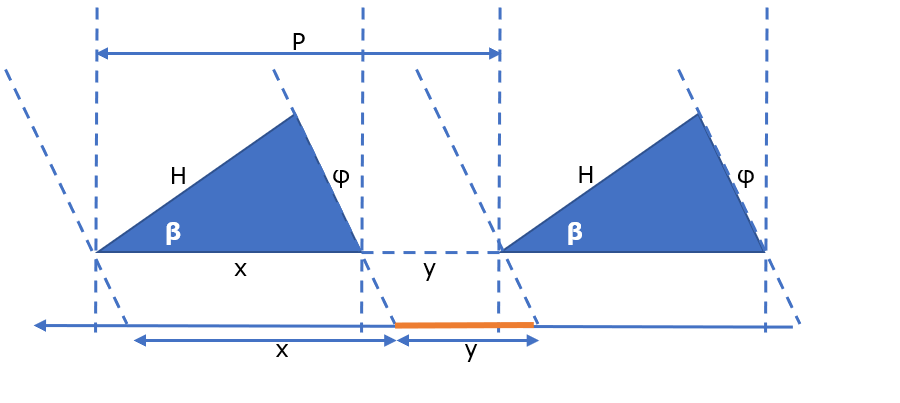
\includegraphics[width=9cm]{2d_infinite_sheds.png}
\caption{Two-dimensional infinitely long PV racks at tilt, $\beta$, each of length $H$, separated by distance $P$.  The vertical dashed lines are parallel to the z-axis, the arrow to the left is the y-axis, and the x-axis points into the page, forming a right-hand coordinate system.  The projection of the solar angle on the y-z plane is $\phi$. The shaded and illuminated regions beneath the racks are shown as $x$ and $y$, respectively.}
\label{fig:2d-infinite-sheds}
\end{figure}

We calculate backside irradiance by treating it as a surface tilted by the supplement of the front surface, and an azimuth that is rotated 180\degree\ around the zenith from the front surface.  The irradiance components for both surfaces can be calculated using any of the transposition models.  Fig. \ref{fig:frontside-transposition} and \ref{fig:backside-transposition} show the irradiance components for the front and back surfaces of a PV rack calculated using several transposition models from pvlib-python \cite{Holmgren2018} with predicted clear sky irradiance at a latitude and longitude of (37.85\degree, -122.25\degree) on the morning of Jan. 1st, 2017.  The front surface is tilted 20\degree\ at an azimuth of 250\degree, so the back surface is tilted at 160\degree\ and the corresponding reference frame is at an azimuth of 70\degree.  The diffuse components are non-zero starting at sunrise at 7:25 PST, but the direct component doesn’t strike the front surface until 8:35 PST because it’s on the back side.

% Fig. 2: frontside transposition
\begin{figure}
\centering
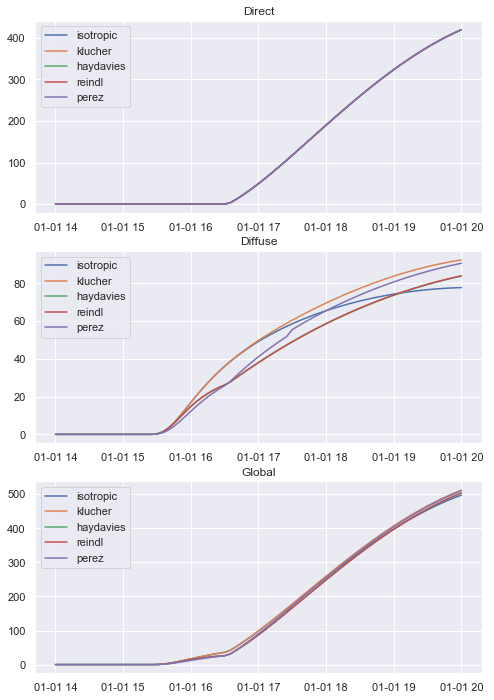
\includegraphics[width=9cm]{frontside_transposition.png}
\caption{Predicted plane of array components using different transposition models on the front surface of a rack tilted at 20\degree\ facing 250\degree\ and located at a latitude and longitude of (37.85\degree, -122.25\degree) on Jan. 1st, 2017.  The top panel shows direct irradiance, the middle shows combined diffuse irradiance from both sky and ground, and the bottom panel shows the total global irradiance on the plane of the array.}
\label{fig:frontside-transposition}
\end{figure}

% Fig. 3: backside transposition
\begin{figure}
\centering
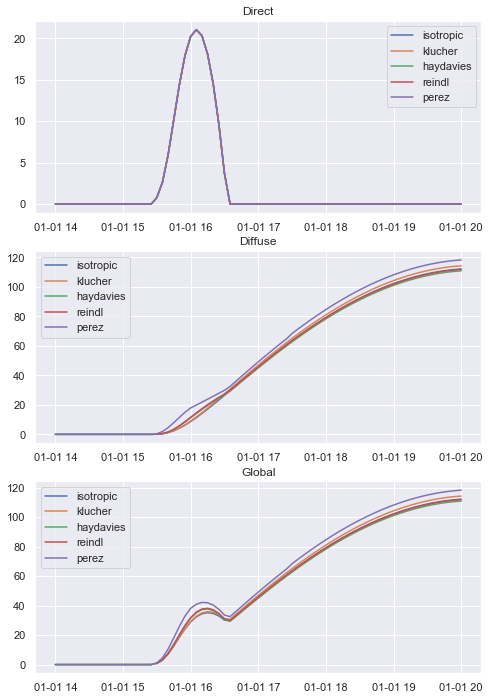
\includegraphics[width=9cm]{backside_transposition.png}
\caption{Predicted plane of array components using different transposition models on the back surface of a rack tilted at 160\degree\ facing 70\degree\ and located at a latitude and longitude of (37.85\degree, -122.25\degree) on Jan. 1st, 2017.  The top panel shows direct irradiance, the middle shows combined diffuse irradiance from both sky and ground, and the bottom panel shows the total global irradiance on the plane of the array.}
\label{fig:backside-transposition}
\end{figure}

Notice in the middle of Fig. \ref{fig:backside-transposition} that the backside diffuse component is significantly overestimated because it doesn’t consider that the PV rack both shades the ground and blocks the sky, therefore reducing incident and reflected irradiance.

\subsection{ Ground Reflection with Shade and Obstructions}
The diffuse components of the irradiance on the front and back surfaces, shown in Fig. \ref{fig:frontside-transposition} and \ref{fig:backside-transposition}, contain contributions from both the sky and ground reflection.  The ground reflection incident on the plane of array, $POA_{gnd}$, assuming no shading and no blocking, is given by the relation in (\ref{eq:POA-gnd}) below with the global horizontal irradiance ($GHI$), the ground albedo ($\rho$), and the view factor from the ground to the PV surface, $F_{gnd,pv} = \frac{\left(1-\cos\beta\right)}{2}$ \cite{Marion2017}.

% Eq. 3: POA_gnd
\begin{equation}
POA_{gnd} = \rho GHI \frac{\left(1-\cos \beta \right)}{2}
\label{eq:POA-gnd}
\end{equation}

The PV rack reduces the ground reflected irradiance both by shading the ground and blocking the sky.  We can account for shade on the ground by calculating the fraction of ground between each pair of rows, $F_{sky,gnd}$, with only incident direct irradiance. The fraction of unshaded ground is expressed in (\ref{eq:Fsky-gnd}) as the ratio $\frac{y}{P}$, with unshaded ground $y$ and row spacing $P$ from Fig. \ref{fig:2d-infinite-sheds}.  The fraction of the shaded ground is then $1-F_{sky,gnd}$.

% Eq. 4: Fsky-gnd
\begin{equation}
F_{sky,gnd} = 1 - \min(0,\ GCR \left| \cos \beta + \sin \beta \tan \phi \right|)
\label{eq:Fsky-gnd}
\end{equation}

The ground coverage ratio, $GCR$, is the ratio of the rack height to spacing, $\frac{H}{P}$, from Fig. \ref{fig:2d-infinite-sheds}.  The projected solar angle on the vertical plane perpendicular to the rows is expressed in (\ref{eq:tan-phi}) using solar zenith, $\theta$, solar azimuth, $\gamma$, and the orientation of the PV surface, $\gamma_{surface}$.

% Eq. 5: tan(phi)
\begin{equation}
\tan \phi = \cos \left(\gamma - \gamma_{surface} \right) \tan \theta
\label{eq:tan-phi}
\end{equation}

As shown in Fig. \ref{fig:ground-sky-vf}, the view of sky from the ground is blocked by the PV panels.  We can account for the blocked sky between each pair of rows by calculating the view factor of the sky from the ground, $F_{x \rightarrow sky}$ given by the angles $\psi_0(x)$ and $\psi_1\left(x\right)$ \cite{Marion2017}.

% Eq. 6: Fx-sky
\begin{equation}
F_{x \rightarrow sky} = \frac{\cos \psi_0\left(x \right) + \cos \psi_1\left(x \right)}{2}
\label{eq:Fx-sky}
\end{equation}

% Fig. 4: ground-sky view factor
\begin{figure}
\centering
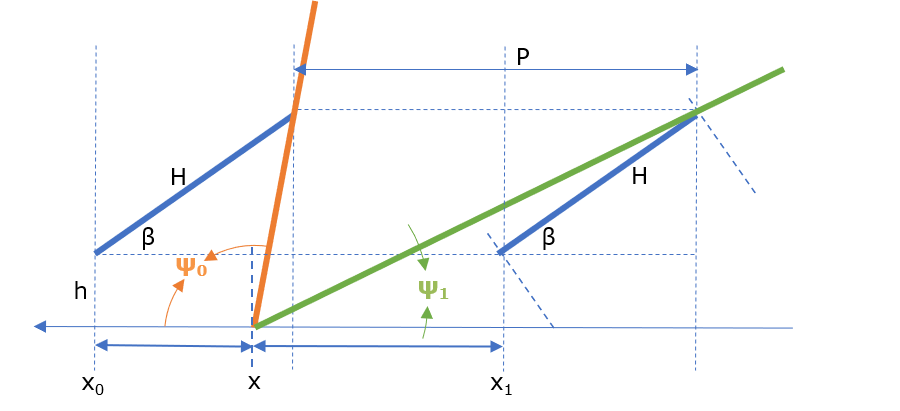
\includegraphics[width=9cm]{ground_sky_vf.png}
\caption{Two dimensional view of a pair of adjacent rows at $x_0$ and $x_1$ separated by spacing $P$, tilted by angle $\beta$, of height $H$, and at height $h$ above the ground.  The view of the sky at point $x$ on the ground is subtended by angles $\psi_0(x)$ and $\psi_1\left(x\right)$.}
\label{fig:ground-sky-vf}
\end{figure}

Note in Fig. \ref{fig:ground-sky-vf} the angles are both measured from the ground in opposite directions.  If one of the angles is replaced with its supplement, the view factor in (\ref{eq:Fx-sky}) would be a difference of cosines instead of the sum, because $\cos \left(\pi - \alpha\right) = -\cos \alpha$.  However, defining the angles this way makes their derivation easier, so for any $x$ the angles are given as follows:

% Eq. 7 & 8: tan(psi)
\begin{equation}
\tan \psi_0 = \frac{\sin \beta^\prime}{\frac{F_x}{GCR^\prime} + \cos \beta^\prime}
\label{eq:tan-psi-0}
\end{equation}

\begin{equation}
\tan \psi_1 = \frac{\sin \beta}{\frac{F_y}{GCR^\prime} + \cos \beta}
\label{eq:tan-psi-1}
\end{equation}

In (\ref{eq:tan-psi-0}), $\beta^\prime$ is the supplement of $\beta$ and $F_x$ is the fraction of the row spacing, $P$, from $x_0$ to $x$, in (\ref{eq:tan-psi-0}) and (\ref{eq:tan-psi-1}), $GCR^\prime=GCR+\frac{h}{P\sin\beta}$ to account for the height of the PV racks above the ground, $h$, and in (\ref{eq:tan-psi-1}), $F_y=1-F_x$ for convenience.

As the PV rack height above the ground, $h$, is increased, the ground near $x_0$ and $x_1$ can see the sky between adjacent rows, although they are blocked by the bottom of the panel closest to that point.  We can derive the limiting angles from the top to the bottom of each row and vice versa, $\psi_{top}\left(x=0\right)$ and $\psi_{bottom}\left(y=0\right)$ in Fig. \ref{fig:nextrow-vf-angles}, and combine the contribution from adjacent rows.  Examining the combined view factors for several heights above the ground, rack tilts, and GCR values, shown in Fig. \ref{fig:Fx-sky-v-tilt-gcr-h}, we observe that the integrated view factor for the space between rows does not vary with height above the ground, only GCR and tilt.  Therefore the zero-height view factor can be used, which simplifies the calculation.  The integrated view factors for the combinations of GCR and tilt are summarized in Table \ref{table1}.

% Fig. 5: next row view factor angles
\begin{figure}
\centering
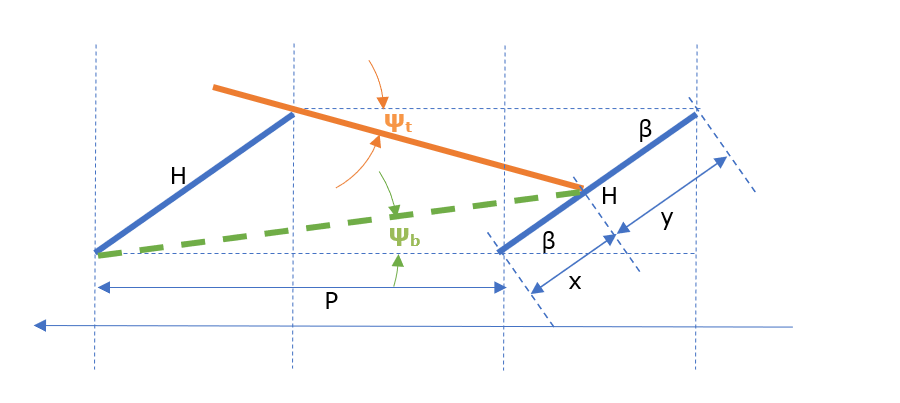
\includegraphics[width=9cm]{next-row-view-factor-angles.png}
\caption{The view of the sky and the ground from the surface of the PV at point $x$ are limited by the angles $\psi_{top}$ and $\psi_{bottom}$ to the top and bottom of the next row.}
\label{fig:nextrow-vf-angles}
\end{figure}

% Fig. 6: Fx-sky vs. tilt, GCR, & h
\begin{figure*}
\centering
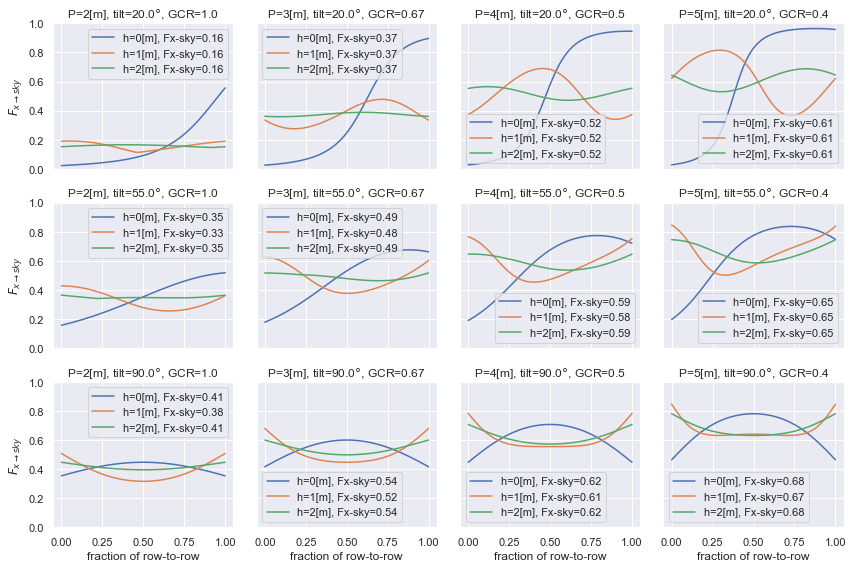
\includegraphics[width=18cm]{Fx-sky_v_tilt_gcr_h.png}
\caption{View factor calculations of $F_{x \rightarrow sky}$ for different combinations of tilt, GCR, and height above the ground.  The view factor is on the vertical axis of each plot and the fraction of the spacing between rows is on the horizontal axis.  The row spacing, $P$, increases from 2 to 5-meters in each plot from the left to the right, and the tilt increases from 20\degree\ to 90\degree\ in each plot from top to bottom.  Each plot shows increasing height above the ground from 0 to 2-meters.  The legend shows the integrated view factor does not vary with height.  The trapezoid rule was used with 100 equally spaced points.}
\label{fig:Fx-sky-v-tilt-gcr-h}
\end{figure*}

% Table I: ground-sky view factor vs. tilt & gcr
\begin{table}
\caption{Ground-Sky View Factor vs. Tilt and GCR}
\centerline{
\vbox{\offinterlineskip
\hrule
% Leading & means preamble template repeats infinitely. p.241 TeX Book.
\halign{&\vrule#&
\strut\quad#\hfil\quad\cr
height2pt&\omit&&\omit&&\omit&&\omit&&\omit&\cr
&Tilt\ /\ GCR&&1.0&&0.67&&0.5&&0.4&\cr
height2pt&\omit&&\omit&&\omit&&\omit&&\omit&\cr
\noalign{\hrule}
height2pt&\omit&&\omit&&\omit&&\omit&&\omit&\cr
&20\degree&&0.16&&0.37&&0.52&&0.61&\cr
&55\degree&&0.35&&0.49&&0.59&&0.65&\cr
&90\degree&&0.41&&0.54&&0.62&&0.68&\cr
height2pt&\omit&&\omit&&\omit&&\omit&&\omit&\cr}
\hrule}}
\label{table1}
\end{table}

We split the GHI into diffuse horizontal irradiance, $DHI$, in the shade, because we assume direct irradiance is only incident on the unshaded ground.  Then the reflected irradiance from the ground with shade and blocked sky, $POA_{gnd,shade}$, incident on the front and back surfaces is the sum from shaded and unshaded ground, where the diffuse ratio is $df=\frac{DHI}{GHI}$, $F_{sky,gnd}$ is the fraction of unshaded ground with incident direct irradiance, and $F_{x \rightarrow sky}$ is the integrated view factor of the sky visible from the ground between the rows.

% Eq. 9: POA_gnd,shade
\begin{equation}
POA_{gnd,shade} = POA_{gnd}\left(F_{sky,gnd} \left(1-df \right) + F_{x \rightarrow sky} df\right)
\label{eq:POA-gnd-shade}
\end{equation}

Note, this still doesn’t account for obstruction by adjacent rows of the view from the front and back PV surfaces to the ground and sky, because the view factor of the ground in (\ref{eq:POA-gnd}) only considers a single row. The next section will consider obstruction by adjacent rows.

Another important consideration is the effect of the width of the sun on the fraction of shaded ground. The radius of the solar disc is about 4.65-milliradians or 0.266\degree\ which would decrease the size of the shadow as the height above the ground of the PV rack was increased. This effect is not considered in the current work.

\subsection{View Factor Obstruction by Adjacent Row}
The bottom of the next row obstructs the view of the ground from the PV surface, and the top of the next row obstructs the view of the sky.  The views from a point, $x$, on the PV surface are limited by the angles, $\psi_{top}$ and $\psi_{bottom}$, from the point to the top and bottom of the next row as shown in Fig. \ref{fig:nextrow-vf-angles}.  The POA components from the ground and sky already account for the view factor without the adjacent row.  The view factor of the ground for a single row was used in (\ref{eq:POA-gnd}), and there's a similar expression for the view factor of the sky, $F_{sky,pv}=\frac{\left(1+\cos\beta\right)}{2}$ \cite{Marion2017}. We need to adjust these view factors to account for the slice from $\beta$ to $\psi$, by the ratio of the blocked and unblocked views.

Adjustment to $F_{gnd,pv}$:

% Eq. 10
\begin{equation}
F_{gnd,pv,row}\left(\psi_{bottom} \right) = \frac{\cos \psi_{bottom} - \cos \beta}{1-\cos\beta}
\end{equation}

Adjustment to $F_{sky,pv}$:

% Eq. 11
\begin{equation}
F_{sky,pv,row}\left(\psi_{top} \right) = \frac{\cos \psi_{top} + \cos \beta}{1+\cos\beta}
\end{equation}

We can derive expressions for the angles to the top and bottom of the next row as a function of an arbitrary position $x$ on the PV surface.

% Eq. 12 & 13
\begin{align}
\tan \psi_{top}\left(x \right) &= \frac{F_x GCR \sin \beta}{1 + F_x GCR \cos \beta}\\
\tan \psi_{bottom}\left(x \right) &= \frac{F_y GCR \sin \beta}{1 - F_y GCR \cos \beta}
\end{align}

Fig. \ref{fig:gnd-front-nextrow}, \ref{fig:gnd-back-nextrow}, \ref{fig:sky-front-nextrow}, and \ref{fig:sky-back-nextrow} show that the ground and sky view factor adjustments are nearly linear from the top to the bottom of the rack.  At the bottom of the PV surface, where $F_x=0$, the ground view factor adjustment is 1, and $\psi_{bottom}=0$.  Then, the ground view factor adjustment decreases by more than 50\% on the front surface in Fig. \ref{fig:gnd-front-nextrow} but less than 10\% on the back surface in Fig. \ref{fig:gnd-back-nextrow}, as $x$ moves to the top of the panel.  At the top of the PV surface, where $F_x=1$, the sky view factor adjustment is 1, and the $\psi_{top}=0$.  Then the sky view factor adjustment decreases by less than 10\% on the front surface in Fig. \ref{fig:sky-front-nextrow}, but more than 50\% on the back surface in Fig. \ref{fig:sky-back-nextrow}, as $x$ moves to the bottom of the panel.

% Fig. 7: ground diffuse on frontside w/nextrow
\begin{figure}
\centering
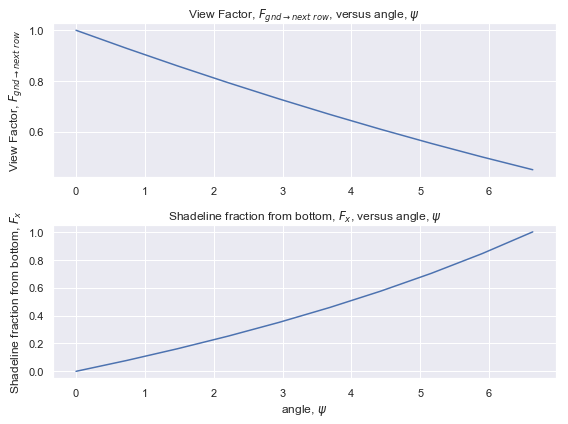
\includegraphics[width=9cm]{ground_diffuse_front_w-next_row.png}
\caption{Ground view factor adjustment and shadeline on the front surface of a rack tilted at 20\degree\ facing 250\degree\ and located at a latitude and longitude of (37.85\degree, -122.25\degree).}
\label{fig:gnd-front-nextrow}
\end{figure}

% Fig. 8: ground diffuse on backside w/nextrow
\begin{figure}
\centering
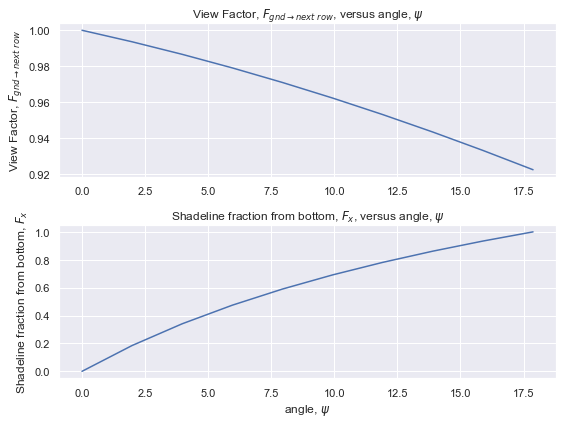
\includegraphics[width=9cm]{ground_diffuse_back_w-next_row.png}
\caption{Ground view factor adjustment and shadeline on the back surface of a rack tilted at 160\degree\ facing 70\degree\ and located at a latitude and longitude of (37.85\degree, -122.25\degree).}
\label{fig:gnd-back-nextrow}
\end{figure}

% Fig. 9: sky diffuse on frontside w/nextrow
\begin{figure}
\centering
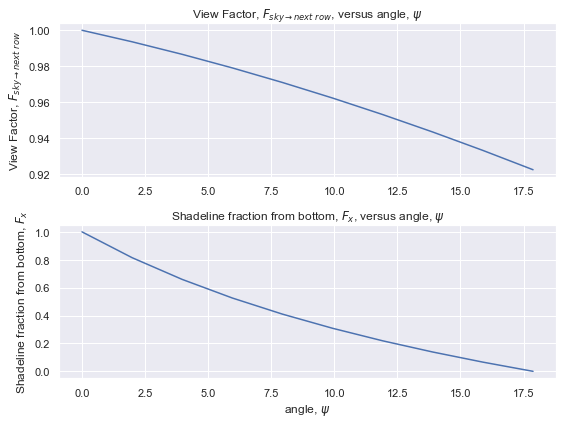
\includegraphics[width=9cm]{sky_diffuse_front_w-next_row.png}
\caption{Sky view factor adjustment and shadeline on the front surface of a rack tilted at 20\degree\ facing 250\degree\ and located at a latitude and longitude of (37.85\degree, -122.25\degree).}
\label{fig:sky-front-nextrow}
\end{figure}

% Fig. 10: sky diffuse on backside w/nextrow
\begin{figure}
\centering
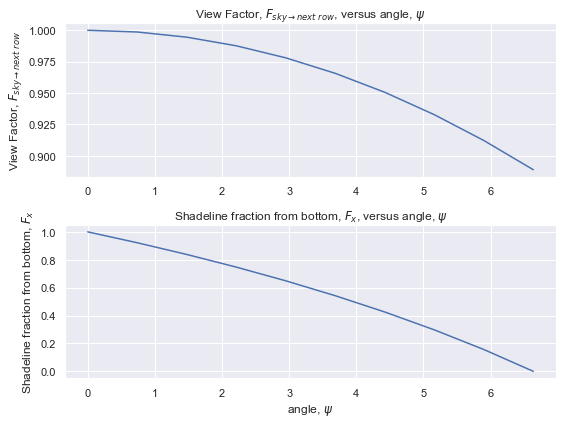
\includegraphics[width=9cm]{sky_diffuse_back_w-next_row.png}
\caption{Sky view factor adjustment and shadeline on the back surface of a rack tilted at 160\degree\ facing 70\degree\ and located at a latitude and longitude of (37.85\degree, -122.25\degree).}
\label{fig:sky-back-nextrow}
\end{figure}

We split the surface into shade and light, integrate over each part, and add them together.  The shadeline, $x_{shade}$, separating shade from light is given by the fraction, $F_x$, of the rack height from the bottom edge of the rack.  The fraction from shadeline to the top of the rack is $F_y = 1 - F_x$. Both $F_x$ and $F_y$ are limited to values between 0 and 1.

% Eq. 14
\begin{equation}
F_{x,shade} = 1 - \frac{1}{GCR\left(\cos \beta + \sin\beta \tan\phi \right)}
\end{equation}

Since the view factors are approximately linear, we estimate the integrals as averages of the view factor adjustments from the endpoints to the shadeline for both the ground and sky to account for the view blocked by the next row.  Recall that at the top of the PV surface the sky view factor adjustment is one, and at the bottom of the PV surface the ground view factor adjustment is also one.

% Eq. 15, 16, 17, 18
\begin{align}
F_{sky,shade} &= \frac{F_{sky,pv,row}\left(x_{shade} \right)+F_{sky,pv,row}\left(F_x=0 \right)}{2}\\
F_{sky,light} &= \frac{F_{sky,pv,row}\left(x_{shade} \right)+1}{2}\\
F_{gnd,shade} &= \frac{F_{gnd,pv,row}\left(x_{shade} \right)+1}{2}\\
F_{gnd,light} &= \frac{F_{gnd,pv,row}\left(x_{shade} \right)+F_{gnd,pv,row}\left(F_x=1 \right)}{2}
\end{align}

We sum the diffuse components for the shaded and unshaded sections, but the direct component is only incident in the unshaded section of the surface, $1-F_x$.

% Eq. 19 & 20
\begin{align}
F_{sky,row} &= F_xF_{sky,shade}+\left(1-F_x\right)F_{sky,light}\\
F_{gnd,row} &= F_xF_{gnd,shade}+\left(1-F_x\right)F_{gnd,light}
\end{align}

% Eq. 20 & 21
\begin{align}
POA_{sky,row} &= POA_{sky,shade}F_{sky,row}\\
POA_{gnd,row} &= POA_{gnd,shade}F_{gnd,row}
\end{align}

% Eq. 22
\begin{equation}
POA_{direct,row} = POA_{direct}\left(1-F_x\right)
\end{equation}

Finally we apply an incidence angle modifier to the direct component and add the direct and diffuse to get the total POA irradiance on each surface.

% Eq. 23 & 24
\begin{align}
POA_{diffuse,row} = POA_{sky,row} + POA_{gnd,row}\\
POA_{global,row} = POA_{direct,row}IAM + POA_{diffuse,row}
\end{align}

An incidence angle modifier for diffuse irradiance is ignored, but could be considered by dividing incident diffuse irradiance into discreet bins by angle of incidence \cite{Marion2017}.

\section{Results}
The bifacial model was integrated into SolarFarmer \cite{Mikofski_8547323} and used to simulate the NIST test array in Gaithersburg, MD \cite{Boyd2017,Boyd2017a,Boyd2017b} with a bifaciality of 80\%, strucural shade of 2\%, and zero transmission.  Electrical mismatch due to non-uniform backside irradiance was ignored.  An equivalent monofacial system was compared to the theoretical bifacial system and both were simulated with varying tilt from 20\degree\ to 40\degree, while all other parameters were constant.  The yields of the theoretical bifacial and equivalent monofacial systems are shown in Fig. \ref{fig:NIST-bifi-v-mono}.  The optimum tilt for the bifacial system was 30\degree\, but the optimium tilt for the monofacial system was 25\degree.  The bifacial gain, defined as $BG=\frac{Y_{bifacial}}{Y_{mono}}-1$, was about 10\% and increased with tilt.

% Fig. 11: NIST bifi vs. mono
\begin{figure}
\centering
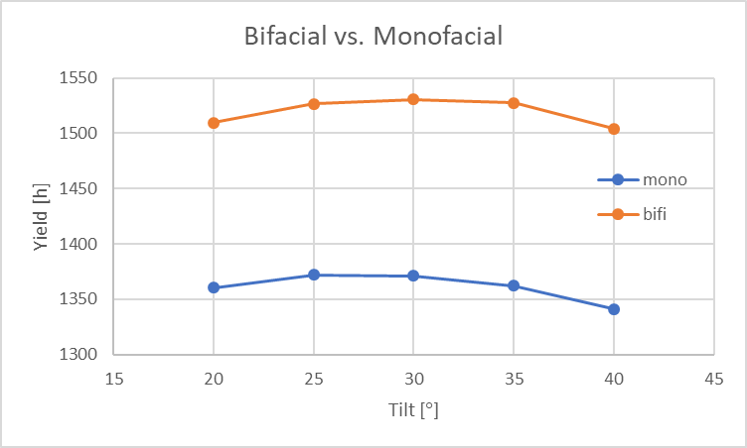
\includegraphics[width=9cm]{NIST_bifi-v-mono.png}
\caption{Theoretical yield from bifacial PV at the NIST test array in Gaithersburg, MD.  Bifaciality was set to 80\% and structural shade was set to 2\%.  Transmission and electrical mismatch due to non-uniform backside irradiance were both ignored.  Tilt was varied from 20\degree\ to 40\degree\ for both bifacial and equivalent monofacial systems.  The maximum yield for bifacial and monofacial occurred at different angles, and the bifacial gain increased with tilt.}
\label{fig:NIST-bifi-v-mono}
\end{figure}



%Further information on LaTeX and TeX can be found in \cite{IEEEhowto:kopka} - \cite{knuth}. 

\section{Conclusion}
A bifacial model similar to existing 2-D view factor models has been integrated into the SolarFarmer PV system performance prediction software.  The model accounts for shade from PV racks on the ground, obstruction of the view factor of the sky from the ground, and blockage of the ground and sky from the PV panels due to adjacent rows.  The view factor of the sky from the ground was estimated using the zero-height rack configuration, because it was observed that rack height above the ground had no effect.  However the width of the sun was neglected, and would be expected to shrink the shadow on the ground as the rack height increased.  View factors from the sky and ground on the PV surfaces were observed to be linear, and therefore linear approximations and weighted averages were used to approximate the effect of adjacent rows.

When the bifacial model was used to simulate the NIST test array in Gaithersburg, MD, the bifacial gain over an equivalent monofacial system was about 10\%.  The bifacial gain was observed to increase with tilt, and it was also observed that the bifacial and monofacial optima occurred at different angles.  This is evidence that a simple bifacial model can be used to estimate bifacial gain, and that there may be different optimal configurations between bifacial and monofacial systems which can be determined using a simple bifacial model.

% conference papers do not normally have an appendix
% use section* for acknowledgment

% trigger a \newpage just before the given reference
% number - used to balance the columns on the last page
% adjust value as needed - may need to be readjusted if
% the document is modified later
%\IEEEtriggeratref{8}
% The "triggered" command can be changed if desired:
%\IEEEtriggercmd{\enlargethispage{-5in}}

% references section

% can use a bibliography generated by BibTeX as a .bbl file
% BibTeX documentation can be easily obtained at:
% http://www.ctan.org/tex-archive/biblio/bibtex/contrib/doc/
% The IEEEtran BibTeX style support page is at:
% http://www.michaelshell.org/tex/ieeetran/bibtex/
\bibliographystyle{IEEEtran}
% argument is your BibTeX string definitions and bibliography database(s)
\bibliography{IEEEabrv,C:/Users/mikm/Projects/pvsc46/bibliography}
%
% <OR> manually copy in the resultant .bbl file
% set second argument of \begin to the number of references
% (used to reserve space for the reference number labels box)

% The following statement makes the two columns on the last page more
% or less of equal length.  Placement of this command is by trial and error.
\vfil\eject

% that's all folks
\end{document}
